\documentclass[12pt]{article}

\usepackage{polski}
\usepackage{fancyhdr}
\usepackage{lastpage}
\usepackage[dvipsnames]{xcolor}
\usepackage{fancyvrb}
\usepackage{graphicx}
\graphicspath{ {./images/} }

\pagestyle{fancy}
\fancyhf{}
\rhead{P. Peszko}
\rfoot{strona \thepage \hspace{1pt} z \pageref{LastPage}}


\title{Gra "Snake" sterowana sztuczną siecią neuronową. Specyfikacja Implementacyjna}
\author{Patryk Peszko}
\date{25 marca 2021}


\begin{document}
	\begin{titlepage}
		\clearpage\maketitle\thispagestyle{empty}
		\maketitle
	\end{titlepage}
	
	\tableofcontents
	\newpage
	\section {Wstęp}
		Dokument ten jest kontynuacją dokumentu pt. "Gra "Snake" sterowana sztuczną siecią neuronową. Specyfikacja Funkcjonalna". W tym dokumencie postaram się opisać sposób w jaki mam zamiar napisać ten program, jak będę go wersjonować oraz z jakich modułów będzie się on składać.
	
	\section {Środowisko deweloperskie}
		\subsection{Parametry komputera}
			- laptop Lenovo Ideapad 720s-14IKB z procesorem m Intel(R) Core(TM) i7-8555U CPU @ 1.80Ghz 2.00Ghz z 8 GB pamięci RAM, działającym na systemie Windows 10 Home wersja 1909
			
		\subsection{Programy wykorzystywane podczas projektu}
			- IntelliJ IDEA Community Edition 2019.3.2 x64 
			
		\subsection{Środowisko kompilacji}
			- Microsoft Windows 10 Home wersja 20H2
			
		\subsection{Standard}
			Projekt pisany będzie zgodny z standardem Java 13.
		
	\section {Zasady wersjonowania}
		Wersje plików wrzucanych na gita będę zaznaczać w tag'ach. Krótkie komentarze, pisane w języku polskim, na temat zmian wprowadzonych w kodzie, będą się znajdować w commit'ach:
		\begin{itemize}
			\item "v n" wersja stabilna gdzie n = { 0, 1, 2, ...}
			\item "v n.m" wersja z drobnymi poprawami gdzie m = { 1, 2, ...}
			\item "v FINAL" ostateczna wersja programu				
		\end{itemize}
	
	\section {Struktura projektu}
		\subsection {Opis modułów}
			Program będzie składał się z wymienionych modułów:
			\begin{itemize}
				\item Neuron.java - pojedynczy neuron
				\item Layer.java - warstwa sztucznej sieci neuronowej
				\item NeuronNetwork.java - cała sieć neuronowa
				\item ListsHolder.java - interfejs
				\item SnakeRunByNeuronNetwork.java - klasa zarządzająca przebiegiem programu
				\item ReadFromFile.java - klasa wczytująca z pliku
				\item WriteToFile.java - klasa zapisująca do pliku
				\item Field.java - komórka planszy
				\item GenerationsGenerator.java - pole gry
				\item Apple.java - jabłko, dziedziczy po Field.java
				\item Graphics.java - zarządza GUI
				\item KeyOperations.java - klasa obsługująca klawiaturę
				\item Snake.java - wąż
				\item Game.java - zarządza grą			
			\end{itemize}
		\subsection{Struktura}
			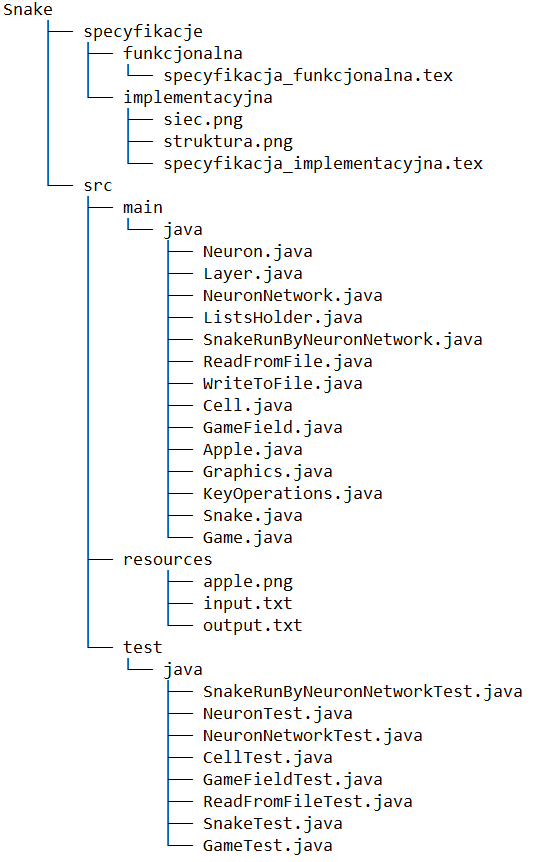
\includegraphics[scale=2]{struktura.png}
		
	\section{Algorytmy i struktury danych}
		Sieć neuronowa będzie przechowywać warstwy w liście liniowej. Warstwy sieci neuronowej będą przechowywać neurony w liście liniowej. Czyli cała sieć będzie przechowywana w liście linowej list liniowych. Komórki, z których będzie się składać wąż, również będą przechowywane w liście liniowej. Listy liniowe i stałe zmienne będą przechowywane w interfejsie.  
		
	\section{Sztuczna sieć neuronowa}
		Zaimplementuję jednokierunkową sieć neuronową. Wszystkie neurony będą mieć tę samą funkcję aktywacji ReLu (rektyfikowana jednostka liniowa). 
		\\
		Pierwszy neuron wyjściowy będzie odpowiedzialny za skręcenie w lewo. Drugi za pójście prosto. Trzeci za skręcenie w prawo. Sieć będzie wybierać neuron o największej wartości i obierać kierunek odpowiadający danemu neuronowi.
		\subsection{Struktura sieci}
			Sieć neuronowa będzie zbudowana z 4 warstw. Pierwsza warstwa 24 neuronów, dwie kolejne będą miały po 18 neuronów a ostatnia będzie się składać z 3 neuronów wyjściowych.
		\subsection{Wizualizacja struktury sieci}	
			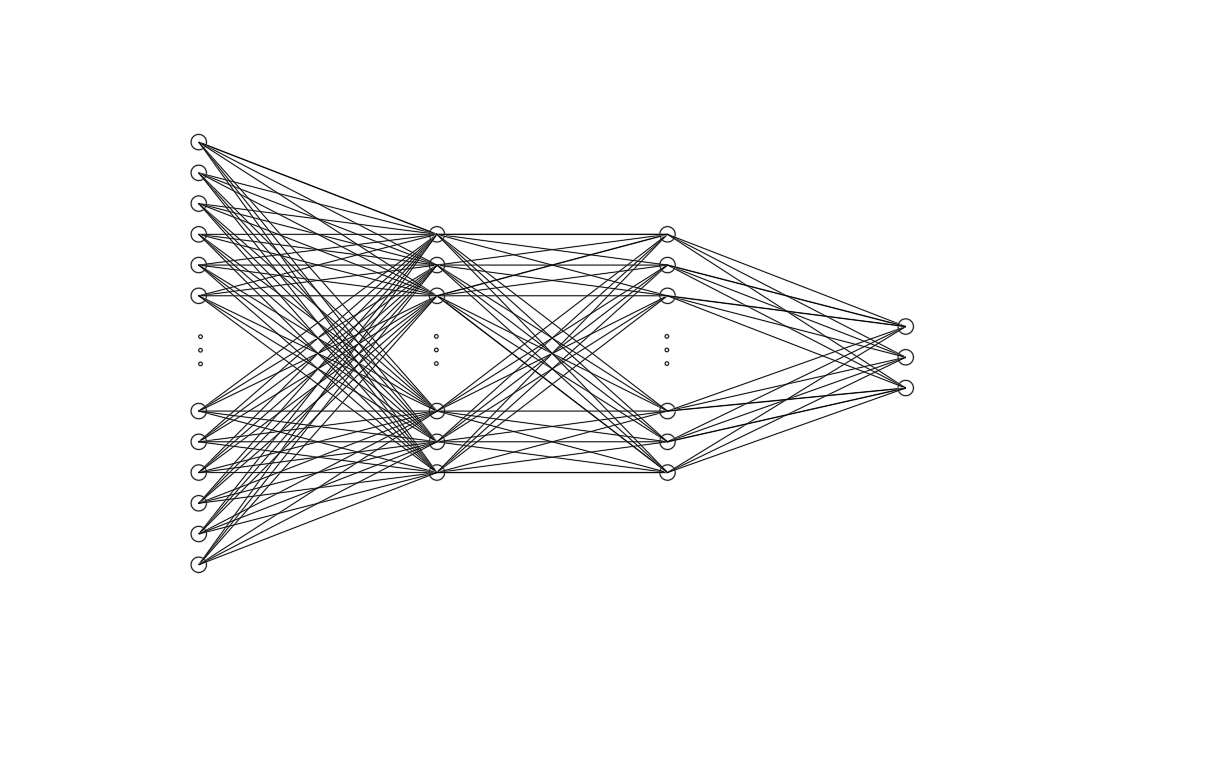
\includegraphics[width=\textwidth]{siec.png}
		\subsection{Nienadzorowane nauczanie sieci}
			Pierwsza generacja węży będzie mieć sieci o współczynnikach losowych. Po zakończeniu gry przez wszystkie węże w danej generacji będzie wybierany najlepszy wąż. Każde jabłko zjedzone przez węża będzie warte 50 punktów a każdy ruch 1 punkt. Wąż będzie startował z możliwością wykonania 100 ruchów, za każde zjedzone jabłko będzie dostawać kolejne 50 ruchów. Po wybraniu najlepszego węża zostanie stworzona kolejna generacja węży, których sieci będą zawierać współczynniki losowe z zakresu \textless 0.9x, 1.1x\textgreater, gdzie x jest współczynnikiem najlepszego węża z poprzedniej generacji. 
	
\end{document}          

        
